\documentclass[UTF8,a4paper]{ctexart}

\usepackage{multicol}
\usepackage{lastpage}
\usepackage{geometry}
\usepackage{mathtools}
\usepackage{tikz}
\usepackage{url}
\usetikzlibrary{positioning, shapes.geometric}

\usepackage{geometry}
\geometry{a4paper,scale=0.7}

\usepackage{subfigure}

\usepackage{fancyhdr}
\pagestyle{fancy}
\lhead{\today}\rhead{Julia 集的分析和探索}
\pagenumbering{arabic}
\lfoot{}
\title{\textbf{\huge{Julia 集的分析和探索}}}
\author{邵盛栋\\信息与计算科学 3200103951}
\date{}
\tikzstyle{decision} = [diamond, aspect = 4, text centered, draw=black]

\usepackage{url}

\makeatletter
\def\url@leostyle{%
	\@ifundefined{selectfont}{\def\UrlFont{\sf}}{\def\UrlFont{\small\ttfamily}}}
\makeatother
\urlstyle{leo}
\begin{document}

	\newcommand{\supercite}[1]{\textsuperscript{\cite{#1}}}
	\maketitle
	\setlength{\oddsidemargin}{ 1cm} 
	\setlength{\evensidemargin}{\oddsidemargin}
	\setlength{\textwidth}{13.50cm}
	\vspace{-0.2cm}

	\begin{center}  \parbox{\textwidth}{  {\heiti 摘~~~要}\quad {\kaishu Julia集是一个在复平面上形成分形的点的集合,以法国数学家加斯顿·朱利亚(Gaston Julia)的名字命名,本文将在研究Julia集的基础上,首先介绍Julia集,并探究其与Mandelbrot集之间的关系,寻找适当的算法并利用C++语言编写程序,最终实现Julia集可视化。}}  
	\end{center}
	
	\section{引言}
	Julia集合可由下式进行反复迭代得到:
	\[f_{c}(z)=z^{2}+c\]
	
	对于固定的复数$ c $,取某一$ z $值(如$ z=z_{0} $),可以得到序列
	\[z_{0},f_{c}(z_{0}),f_{c}(f_{c}(z_{0})),f_{c}(f_{c}(f_{c}(z_{0}))),\dots\]
	
	这一序列可能反散于无穷大或始终处于某一范围之内并收敛于某一值。我们将使其不扩散的$ z $值的集合称为Julia集合。
	\section{数学理论}
	\subsection{背景}
	Julia集以法国数学家Gaston Julia的名字命名,他在1915年研究了它们的性质,并在1918年发表了他的著名论文:\textbf{Mémoire sur l'itération des fonctions rationnelles}。虽然Julia集现在与$ z_{n+1}=z_{n}^{2}+c $有关,但Julia感兴趣的是更一般表达式的迭代性质,即
	\[z^{4}+\dfrac{z^{3}}{z-1}+\dfrac{z^{2}}{z^{3}+4z^{2}+5}+c\]
	由$ z_{n+1}=z_{n}^{2}+c $定义的Julia集合可以有各种形状,c的一个小变化可以极大地改变Julia集合。1979年,在计算机的帮助下,B.B.Mandelbrot研究了Julia集,试图对所有可能的形状进行分类,并提出了一个新的形状: Mandelbrot集\cite{douady1986julia}。
	\subsection{与Mandelbrot集之间的关系}
	由于Mandelbrot集合的定义,在给定点上Mandelbrot集合的几何与对应的Julia集合的结构之间有密切的对应关系。换句话说,Mandelbrot集合形成了Julia集合的一种索引。\cite{lei1990similarity}Julia集合要么是连通的,要么是断开的,从Mandelbrot集合内选择的c值是连通的,而从Mandelbrot集合外选择的c值是断开的。这些不相连的集合通常被称为$ dust $,它们由独立的点组成,不管它们以什么分辨率被观察\cite{Juliaset}。
	\section{算法}
	算法如流程图\ref{fig:1}所示
	\begin{figure}[htpb]
		\centering
		\begin{tikzpicture}[node distance=16pt]
			\node[draw, rounded corners]                        (start)   {开始};
			\node[draw, below=of start]                         (step 1)  {构建一个宽度$ \times $高度为$ 1500\times1500 $的位图};
			\node[draw, below=of step 1]                        (step 2)  {定义函数\verb|write_header()|和\verb|write_pixel()|,实现对像素点颜色属性的赋值};
			\node[draw,decision, below=of step 2]     (step 3)  {取复数z,利用函数\verb|julia()|判断z是否收敛};
			\node[draw, below=of step 3]     (choice1)  {z在规定迭代次数内收敛};
			\node[draw, right=25pt of choice1]     (choice2)  {z在规定迭代次数内发散($ |z|\textgreater 2 $)};
			\node[draw, below=of choice1]     (color1)  {取灰度\verb|intensitive|$ \in [0,1)$};
			\node[draw, below=of choice2]     (color2)  {返回1,取黑色};
			\node[draw, below=of color1]     (result)  {将RGB值赋值到与复数z对应的像素点};
			\node[draw, below=of result]     (again)  {改变复数z的值};
			\node[draw, below=of again]     (output)  {输出位图pbm};
			\node[draw, rounded corners, below=of output]     (end)   {结束};
			\coordinate (point1) at (-160pt, -291pt);
			
			\draw[->] (start)  -- (step 1);
			\draw[->] (step 1) -- (step 2);
			\draw[->] (step 2) -- (step 3);
			\draw[->] (step 3) -- (choice1);
			\draw[->] (step 3) -- (step 3-|choice2) -> (choice2);
			\draw[->] (choice1) -- (color1);
			\draw[->] (choice2) -- (color2);
			\draw[->] (color1) -- (result);
			\draw[->] (color2) -- (color2|-result) -> (result);
			\draw[->] (result) -- (again);
			\draw (again) -- (point1);
			\draw [->] (point1) |- (step 3);
			\draw[->] (again) -- (output);
			\draw[->] (output) -- (end);
			
		\end{tikzpicture}
		\caption{具体算法}
		\label{fig:1}
	\end{figure}
	\newpage
	\section{数值算例}
	当我们取不同的复数c的值时,我们能够得到不同的Julia集,这些Julia集大小不同,形状各异,当取某些特定的c的值的时候,对应的Julia集会形成一个连通的区域。执行以下命令可得到相应的pbm图像:
	\begin{verbatim}
		./bin/juliaset -0.4 0.6 picture1.pbm
		./bin/juliaset -0.8 0.156 picture2.pbm
		./bin/juliaset 0.28 0.01 picture3.pbm
		./bin/juliaset 0.3 0.5 picture4.pbm
	\end{verbatim}
	以下是取不同的c时,对应的Julia集的图像:
	\begin{figure}[ht]
		\centering
		\subfigure[$ c=-0.4+0.6i $]{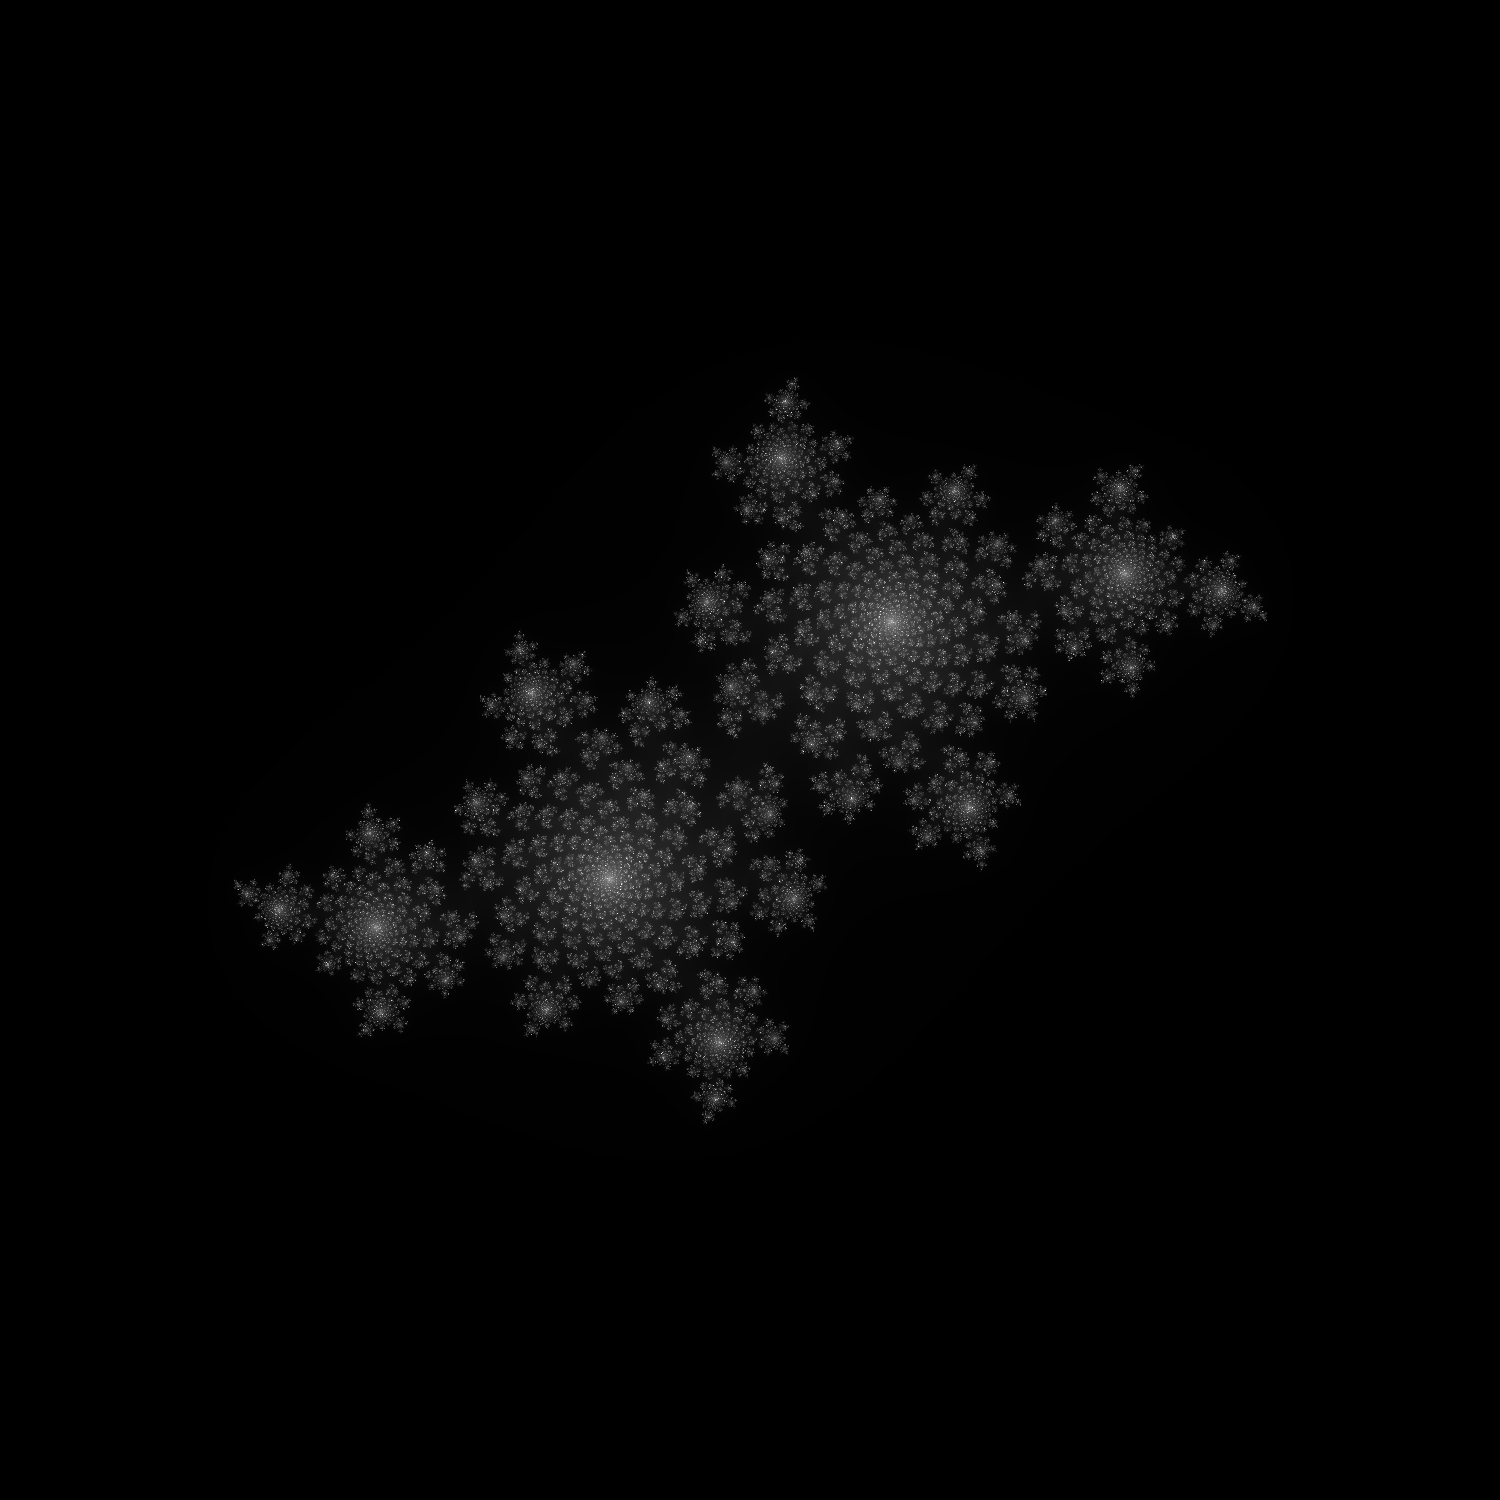
\includegraphics[width=0.4\linewidth]{../image/picture1}}
		\subfigure[$ c=-0.8+0.156i $]{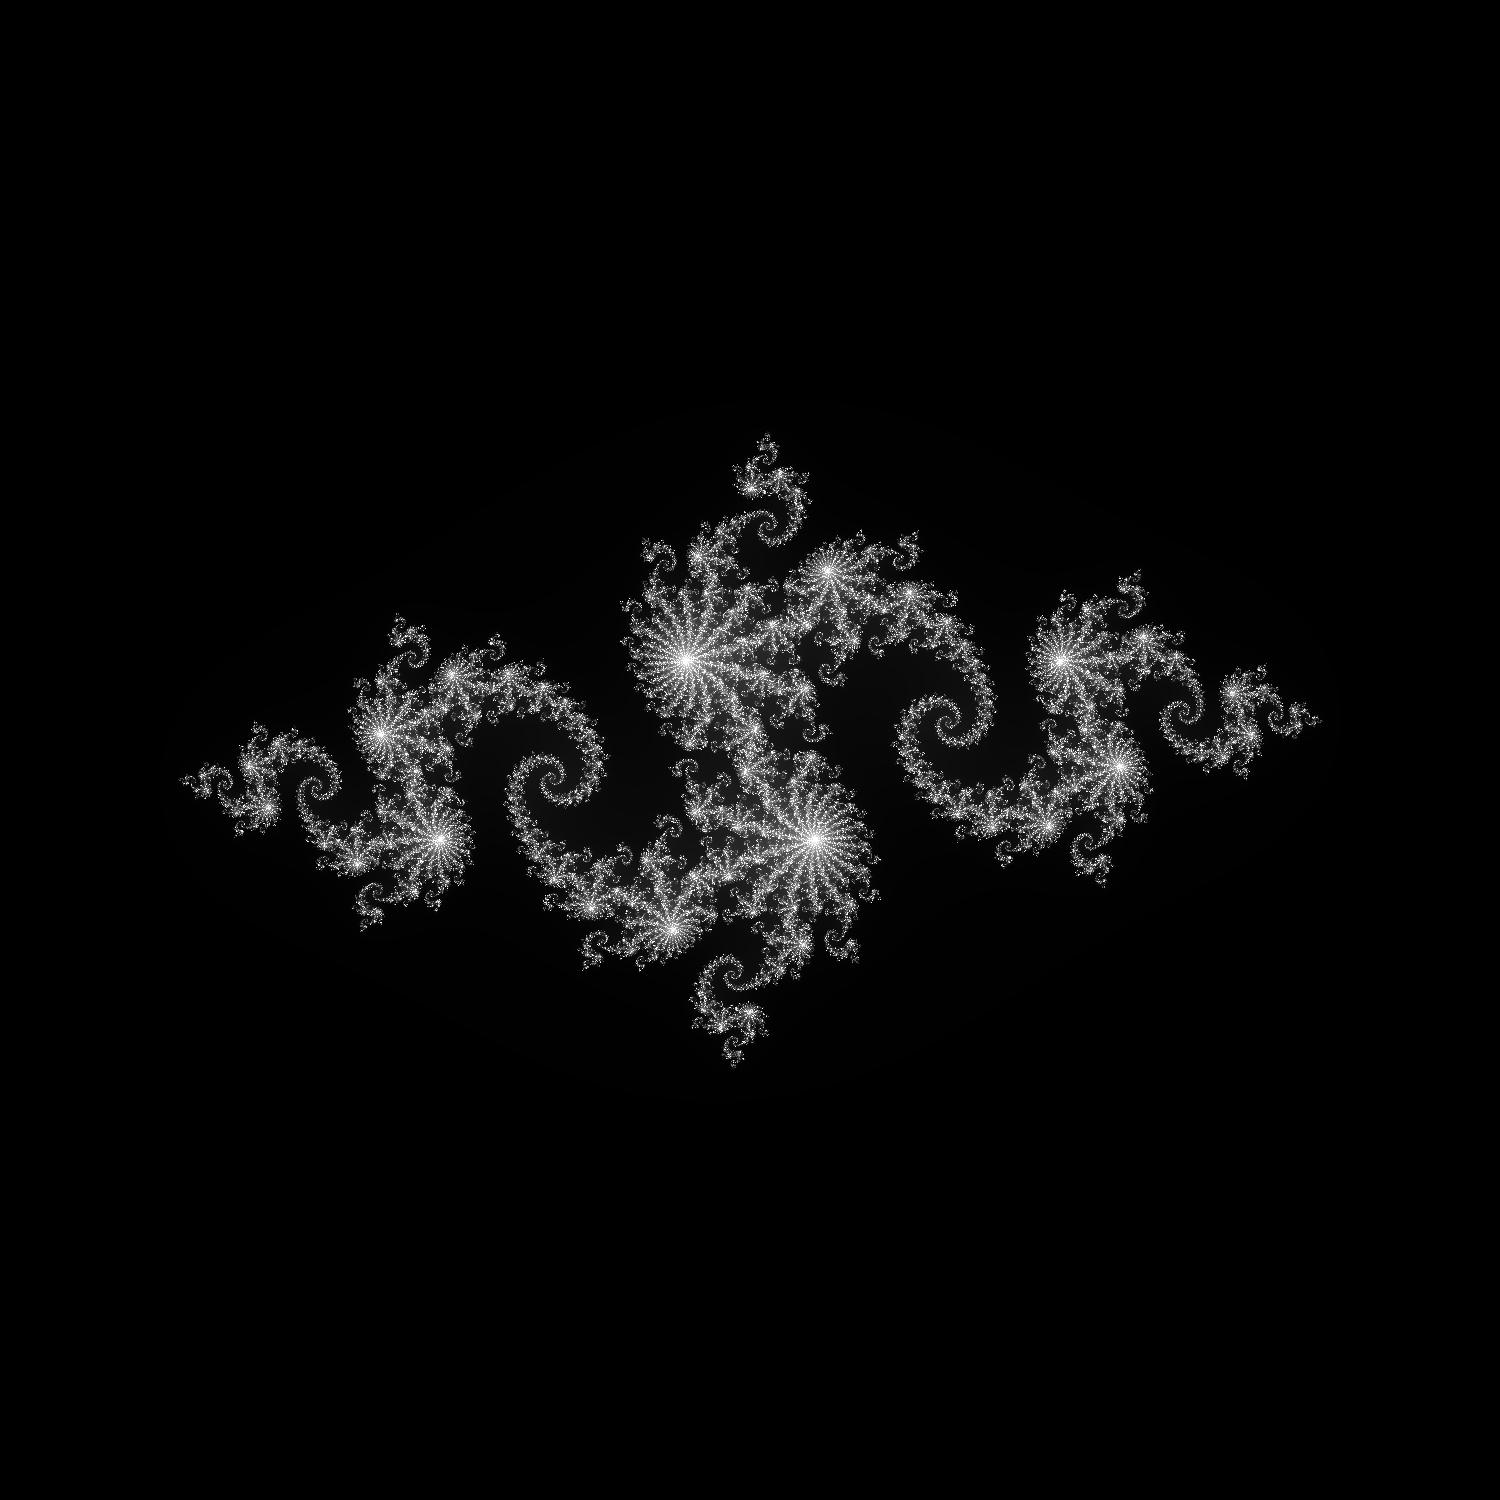
\includegraphics[width=0.4\linewidth]{../image/picture2}}
	\end{figure}
	\begin{figure}[ht]
		\centering
		\subfigure[$ c=0.28+0.01i $]{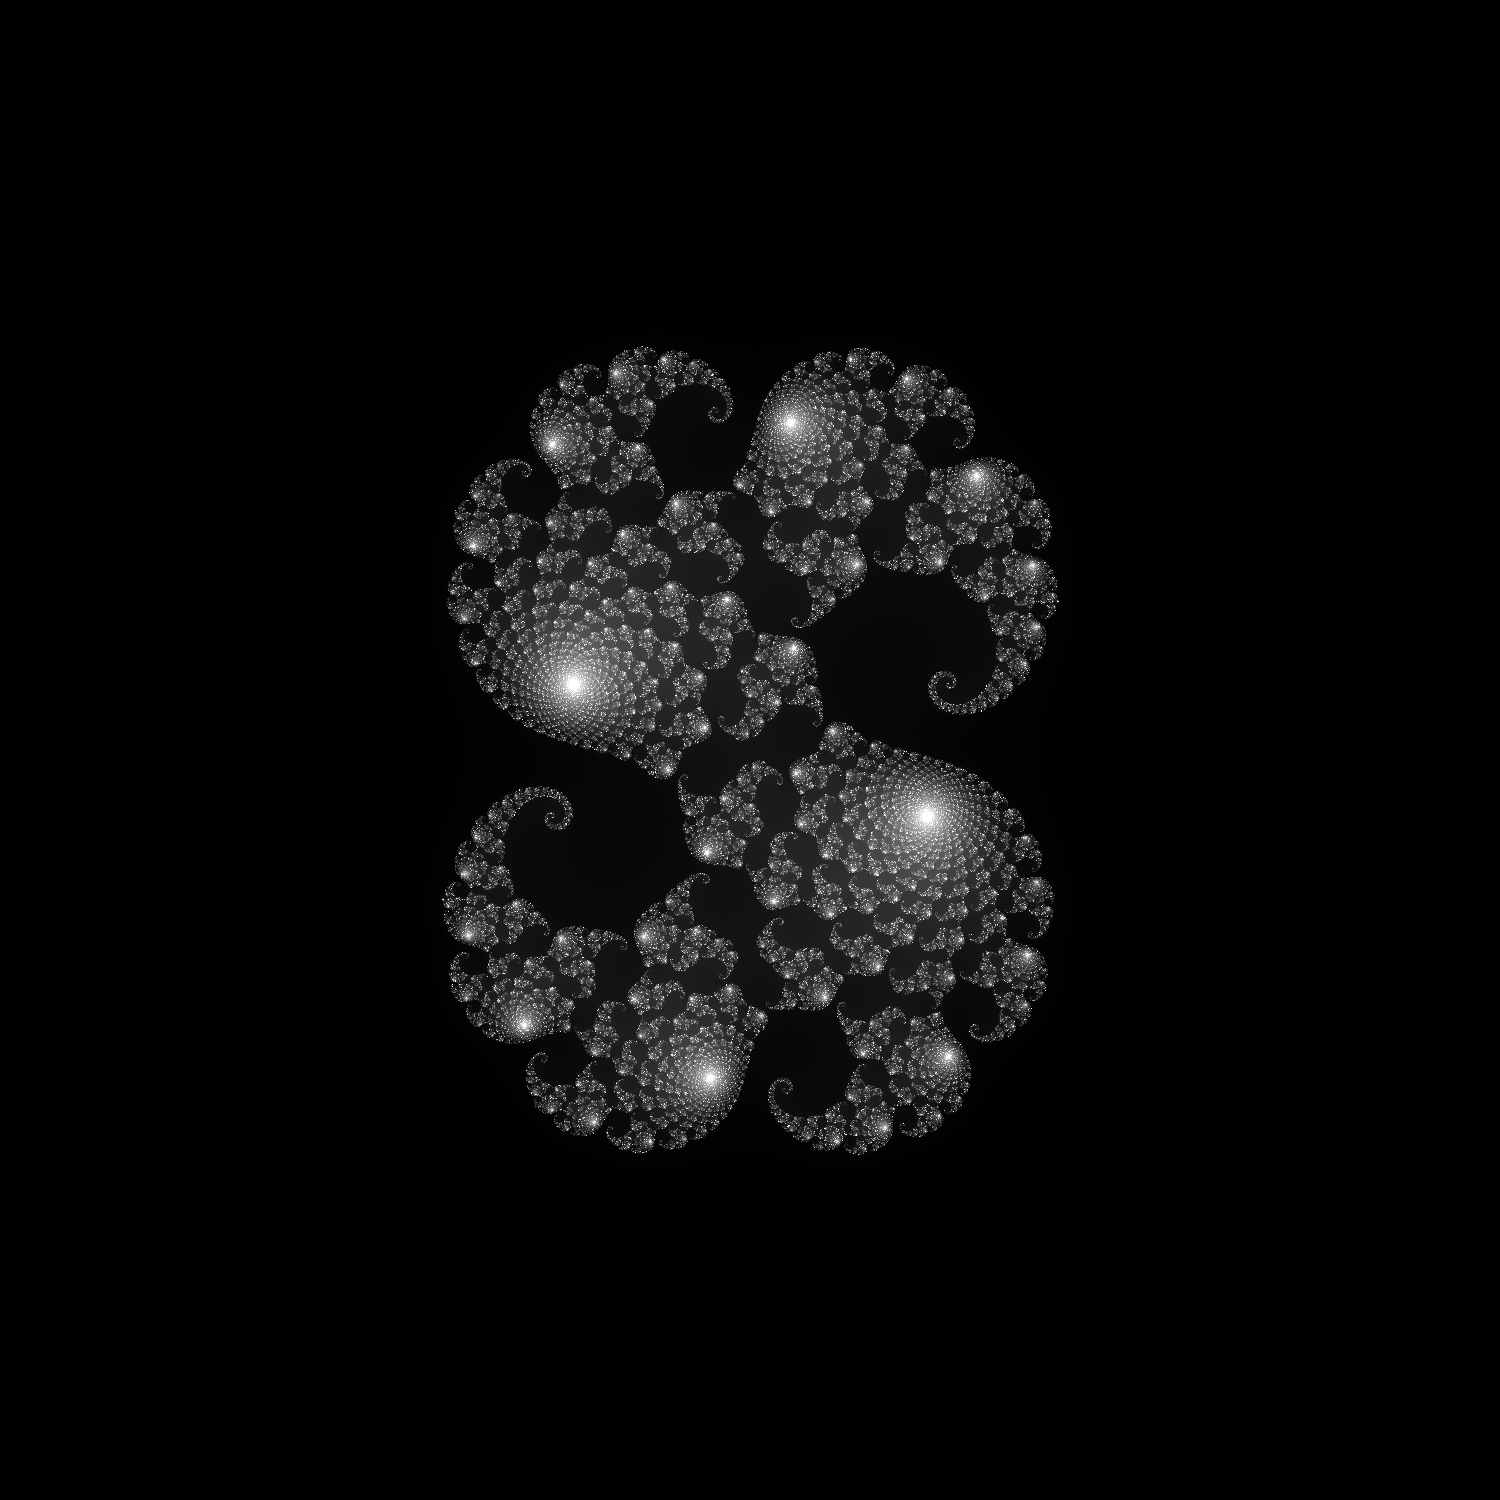
\includegraphics[width=0.4\linewidth]{../image/picture3}}
		\subfigure[$ c=0.3+0.5i $]{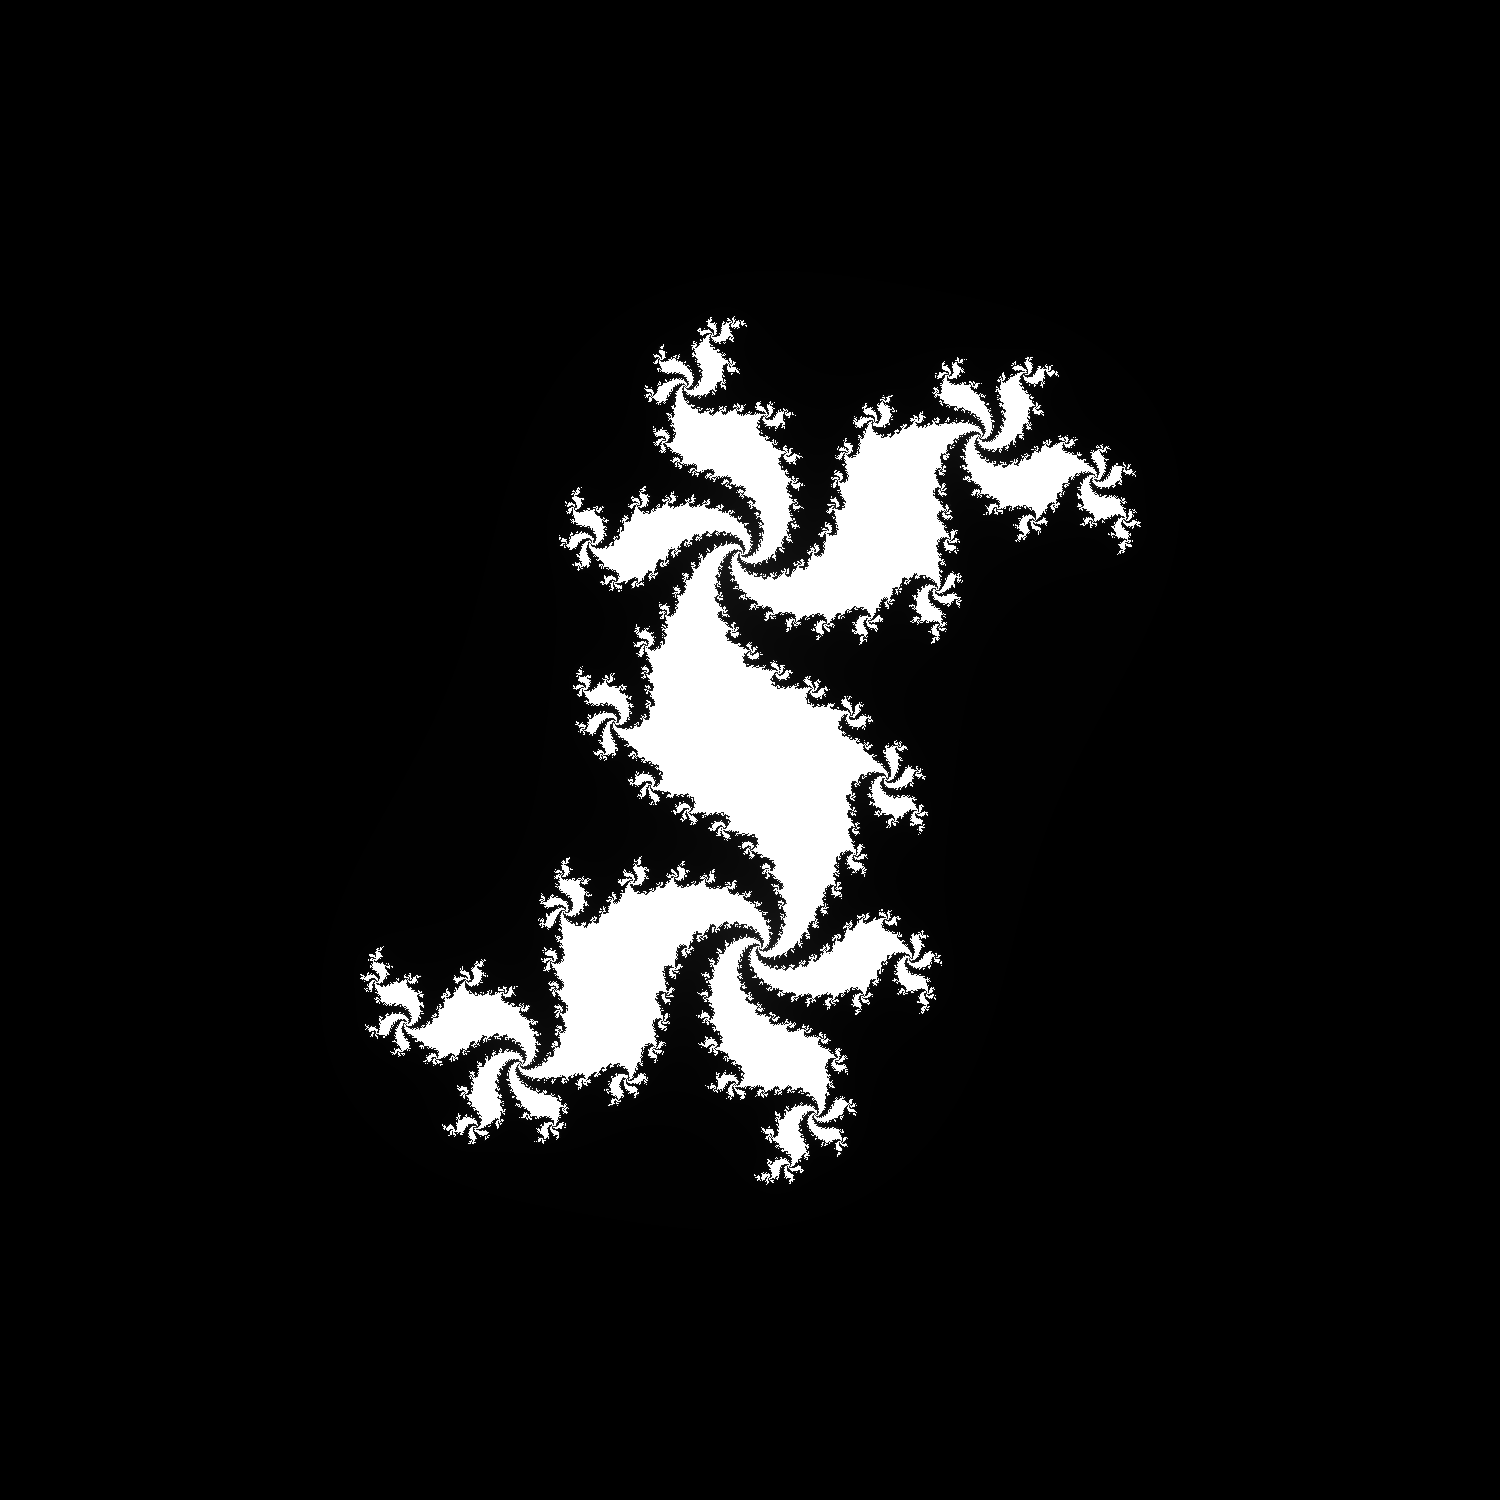
\includegraphics[width=0.4\linewidth]{../image/picture4}}
	\end{figure}
	\newpage
	\section{结论}
	Julia集的中c的不同取值可反映出复数z不同的发散程度,本文中的代码将复数z收敛与发散两种不同情况进行区分,并赋予不同的颜色,由此得到不同的美丽的图案。在此基础上,我们仍可以通过改变维数以及改变c的值,得到一些新的研究思路与方法,发现复变函数中“分形”之美。
	
	\bibliographystyle{unsrt}
	\bibliography{literature}
\end{document}
